\chapterpicture{header_08}
\chapter{Terapia del dolore}

Il dolore\ft{Certe tipologie di dolore possono essere psicosomatici, che sono causati dalle emozioni.}
è definito come

\begin{quoting}
Una gradevole esperienza sensoriale ed emotiva, associata ad un effettivo o potenziale danno tissutale o comunque descritto come tale
\end{quoting}

Il dolore si può dividere in due categorie

\begin{itemize}
\item
\emph{dolore acuto:} è una risposta ad uno stimolo, che allerta il
corpo al pericolo. Per questo viene definito come ``dolore utile'\,',
in quanto permette di riconoscere una patologia in corso.
\item
\emph{dolore cronico:} può derivare da un dolore acuto persistente, ma
molto più spesso è dovuto ad altre patologie note, su cui non si può
intervenire. Basti pensare a certe tipologie di tumore. È quindi un
``dolore inutile'\,' in quanto non è direttamente legato alla
patologia in corso e deve essere trattato in modo diverso.
\end{itemize}

Certi dolori cronici possono venire trattati in modo completo, non solo
con interventi, ma anche con approcci psicologici. Spesso, queste
malattie, comportano degli stati depressivi, che quindi possono essere
trattati con dei farmaci antidepressivi. Altre volte è necessario andare
a bloccare la percezione del dolore e quindi si utilizzano dei farmaci
anestetici

Le classi farmaceutiche per trattare il dolore sono quattro:

\begin{itemize}
\item
Farmaci anti infiammatori
\item
Farmaci analgesici oppioidi
\item
Anestetici locali
\item
Anestetici generali
\end{itemize}

Noi partiremo dai farmaci antiinfiammatori. Il dolore può essere dovuto
a possibili infiammazioni, però può anche essere dovuto a altre
patologie, che riguardano altri organi. In questo caso, il dolore verrà
trattato come proveniente da infiammazioni.

\chapterpicture{header_09}
\chapter{Farmaci antinfiammatori}
\markboth{Farmaci antinfiammatori}{\printitle}

Lo schema generale di un farmaco può essere visto nello specifico, per
lo stato patologico perturbato, che è perturbato da una risposta
infiammatoria. Questo stato patologico si riferisce ad uno stato dove
l'infiammazione crea dei sintomi sufficientemente elevati da
compromettere la quotidianità.

Ci possono essere anche altri sintomi, oltre al dolore, come la febbre.

Il nostro organismo è soggetto a stati infiammatori, però alcuni si
risolvono intervenendo dall'esterno, mentre altri sono molto meno gravi.

In questo caso, la risposta infiammatoria compromette la quotidianità,
quindi è necessario intervenire dall'esterno per ripristinare lo stato
biologico.

Nel caso dell'infiammazione, le macchine molecolari sono le COX
(ciclocarboossigenasi), che è una classe di enzimi. Esistono la COX-1 e
la COX-2, che sono delle isoforme, che differiscono tra di loro in
struttura.

\fullpicture*{17_001}{Spazio chimico, spazio biologico e spazio patologico.}

L'attività enzimatica è la stessa, però sono presenti in due occasioni
diverse. Uno è presente nello stato biologico sano, infatti serve anche
per mantenere l'omeostasi. L'altro invece è presente solo se si è in
presenza di uno stato infiammatorio.

\marginbox*{C'è una certa selettività tra COX-1 e COX-2; sono stati utilizzati diversi farmaci}

Ci sono diverse classi di farmaci antiinfiammatori:

\begin{itemize}
\item
Cortisonici, o farmaci cortisonici.
\item
FANS, ovvero \emph{Farmaci Antiinfiammatori Non Steroidei}
\end{itemize}

I farmaci cortisonici verranno solo accennati, per vedere la differenza
di attività con i FANS.

\marginbox*{
I FANS sono facilmente accessibili alle persone; sono medicinali di automedicazione, in quanto sono molto sicuri. Comunque questi farmaci presentano degli effetti collaterali, che comunque sono importanti se utilizzati scorrettamente o per troppo tempo}

I FANS sono somministrati per via orale, per la facilità di assunzione. I
FANS sono solitamente assunti a stomaco pieno. Inoltre i FANS sono
utilizzati per l'infiammazione acuta e non cronica, quindi non sono
utilizzati per molto tempo.

Questo tipo di farmaci serve per alleviare i sintomi dell'infiammazione.
Il sistema immunitario lavora per risolvere lo stato patologico; i FANS
servono solo per risolvere il dolore.

Le cause dell'infiammazione possono essere diverse:

\begin{itemize}
\item
\emph{Contatto con agenti infettivi}, come batteri,
virus\ft{Come il virus dell'influenza. L'assunzione di FANS serve per contrastare i sintomi, senza curare},
funghi o parassiti. Non tutti i batteri però causano infiammazione. I
batteri possono rilasciare delle sostanze nell'organismo, che sono
dette tossine, e che vanno a peggiorare lo stato patologico.
\item
\emph{Agenti immunologici}, come le reazioni allergiche causate dal
legame tra antigene e anticorpo. La risposta allergica è legata a un
processo infiammatorio.
\item
\emph{Agenti fisici}, come caldo, freddo, esposizione a radiazioni o
trauma meccanico.
\item
\emph{Agenti chimici}, come veleni organici o inorganici, come
l'inquinamento atmosferico.
\item
\emph{Materiali inerti}, come corpi estranei.
\item
\emph{Stress}
\end{itemize}

I segni dell'infiammazione sono cinque e sono:

\begin{itemize}
\item
\emph{Rossore:} dovuto all'allargarsi dei vasi sanguigni.
\item
\emph{Edema:} l'infiammazione causa del gonfiore, in quanto le cellule
del sistema immunitario si concentrano.
\item
\emph{Calore:} può essere febbre, piuttosto che un calore locale,
sempre per lo stesso motivo del rossore.
\item
\emph{Dolore}
\item
\emph{Perdita di funzionalità}: avviene nei casi più gravi.
\end{itemize}

Questi cinque segnali sono stati identificati nel passato. Queste
sintomatologie sono definite \emph{punti cardinali} dell'infiammazione

L'infiammazione può essere un evento acuto o cronico:

\begin{itemize}
\item
L'infiammazione acuta avviene a seguito di uno stimolo del sistema
immunitario, quindi vengono reclutate tutte le cellule immunitarie,
che si occuperanno di difendere l'organismo. Questo causa
l'infiammazione, in quanto il processo di difesa porta alla formazione
di scorie, che dovranno essere eliminate. Questo stato si risolve in
poco tempo.
\item
Se il sistema immunitario non è in buona salute, oppure
l'infiammazione è grave, quindi si protrae nel tempo, i cicli si
protraggono nel tempo. L'infiammazione tende a cronicizzare.
\end{itemize}

\subsection{Metabolismo dell'acido arachidonico}

La risposta infiammatoria nasce dall'acido
arachidonico\ft{L'acido arachidonico è una molecola normalmente presente nelle membrane fosfolipidiche e viene accumulata/sintetizzata in grandi quantità.},
non perché questo sia direttamente una sostanza infiammatoria, ma per
via dei suoi metaboliti

Nel momento in cui si è in presenza di uno stato patologico, alcuni
enzimi, detti \emph{fosfolipasi}, che idrolizzano l'acido arachidonico
presente nelle membrane e lo liberano.

L'acido arachidonico libero viene in seguito metabolizzato da altri
enzimi, ovvero \emph{ciclossigenasi} e \emph{lipossigenasi}. Questi
enzimi liberano i mediatori dell'infiammazione, ovvero

\begin{itemize}
\item
Prostaglandine
\item
Prostacicline
\item
Trombossani
\end{itemize}

Ogni mediatore ha un effetto diverso, come si vede nell'immagine \ref{fig:17:AcAra}

\fullpicture{17_002}{Metabolismo dell'acido arachidonico}{fig:17:AcAra}

Non tutte le prostaglandine hanno un effetto pro-infiammatorio, ma
vengono usate anche dallo stato sano. Ad esempio, le prostaglandine E
venegono espresse per ridurre la secrezione di acido gastrico, favorendo
la produzione del muco.

\marginbox*{
L'effetto collaterale dei FANS, che vanno a diminuire la produzione di prostaglandine, è quello di aumentare la secrezione acida, portando quindi ad ulcerazione, se assunte per troppo tempo.\\
In secondo luogo, si ha una tossicità renale, in quanto i reni vengono sovrastimolati.
}

Andando a interagire con alcuni punti del metabolismo dell'acido
arachidonico, si va a ridurre l'infiammazione, ma anche a ridurre delle
reazioni che normalmente servono per mantenere lo stato stazionario.

Tutti i mediatori dell'infiammazione sono eicosanoidi, ovvero sono dei
acidi grassi insaturi formati da venti atomi di carbonio.

\begin{figure}[H]
    \centering
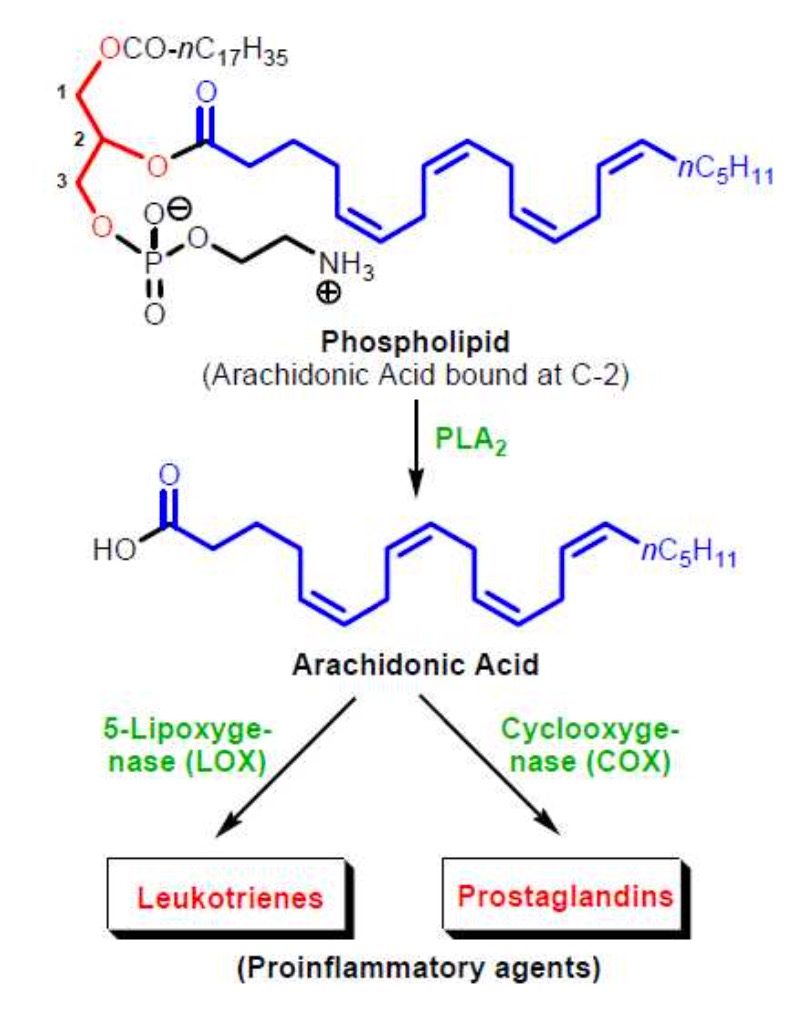
\includegraphics[width=0.5\textwidth]{17_003}
\end{figure}

L'acido arachidonico è anche il precursore di mediatori che servono per
risolvere l'infiammazione. È per questo che c'è una riserva nella
membrana
cellulare\ft{Per questo è necessario assumere molti grassi omega-3 e omega-6.}.
Nel momento in cui si è in presenza di uno stimolo infiammatorio, la
fosfolipasi A2 viene attivata e causa l'idrolisi dell'acido arachidonico
dal fosfolipide, che quindi diventa disponibile per diventare un
mediatore dell'infiammazione

L'acido arachidonico è un acido grasso polinsaturo della famiglia degli
omega-6. Questo acido viene sintetizzato a partire dall'acido linoleico.
Le instaturazioni (tutte cis) determinano una struttura ben precisa per
questa molecola.

Questa molecola è presente nelle membrane cellulari in quanto ha un
\(\log{} P\) pari a 6.99, il che lo rende molto propenso a entrare e
rimanere nella membrana. Per uscire dalla membrana, l'acido arachidonico
deve entrare nel sito attivo delle fosfolipasi.



In seguito, l'acido arachidonico libero entra nelle ciclossigenasi, per
trasformarsi nei mediatori dell'infiammazione.

\marginbox*{La catena respiratoria non serve soltanto per mantenere in vita le cellule, ma serve anche per altre macchine molecolari}

La ciclossigenasi ha due attività catalitiche, ovvero ciclizza e
ossigena la molecola. L'ossigenazione necessita di un agente ossidante,
ovvero l'ossigeno, che è presente molto abbondantemente nelle cellule.
Avviene quindi una reazione redox, che è mediata da un cofattore,
ovvero l'eme.

L'ossigeno molecolare viene ridotto
dall'eme\ft{L'eme è contenuto all'interno nella ciclossigenasi ed è vicino al sito attivo. Il vero e proprio catalizzatore è lo ione \ce{Fe^{2+}} presente nell'eme.},
e diventa uno ione superossido \ce{O2-}.

\begin{figure}[H]
    \centering
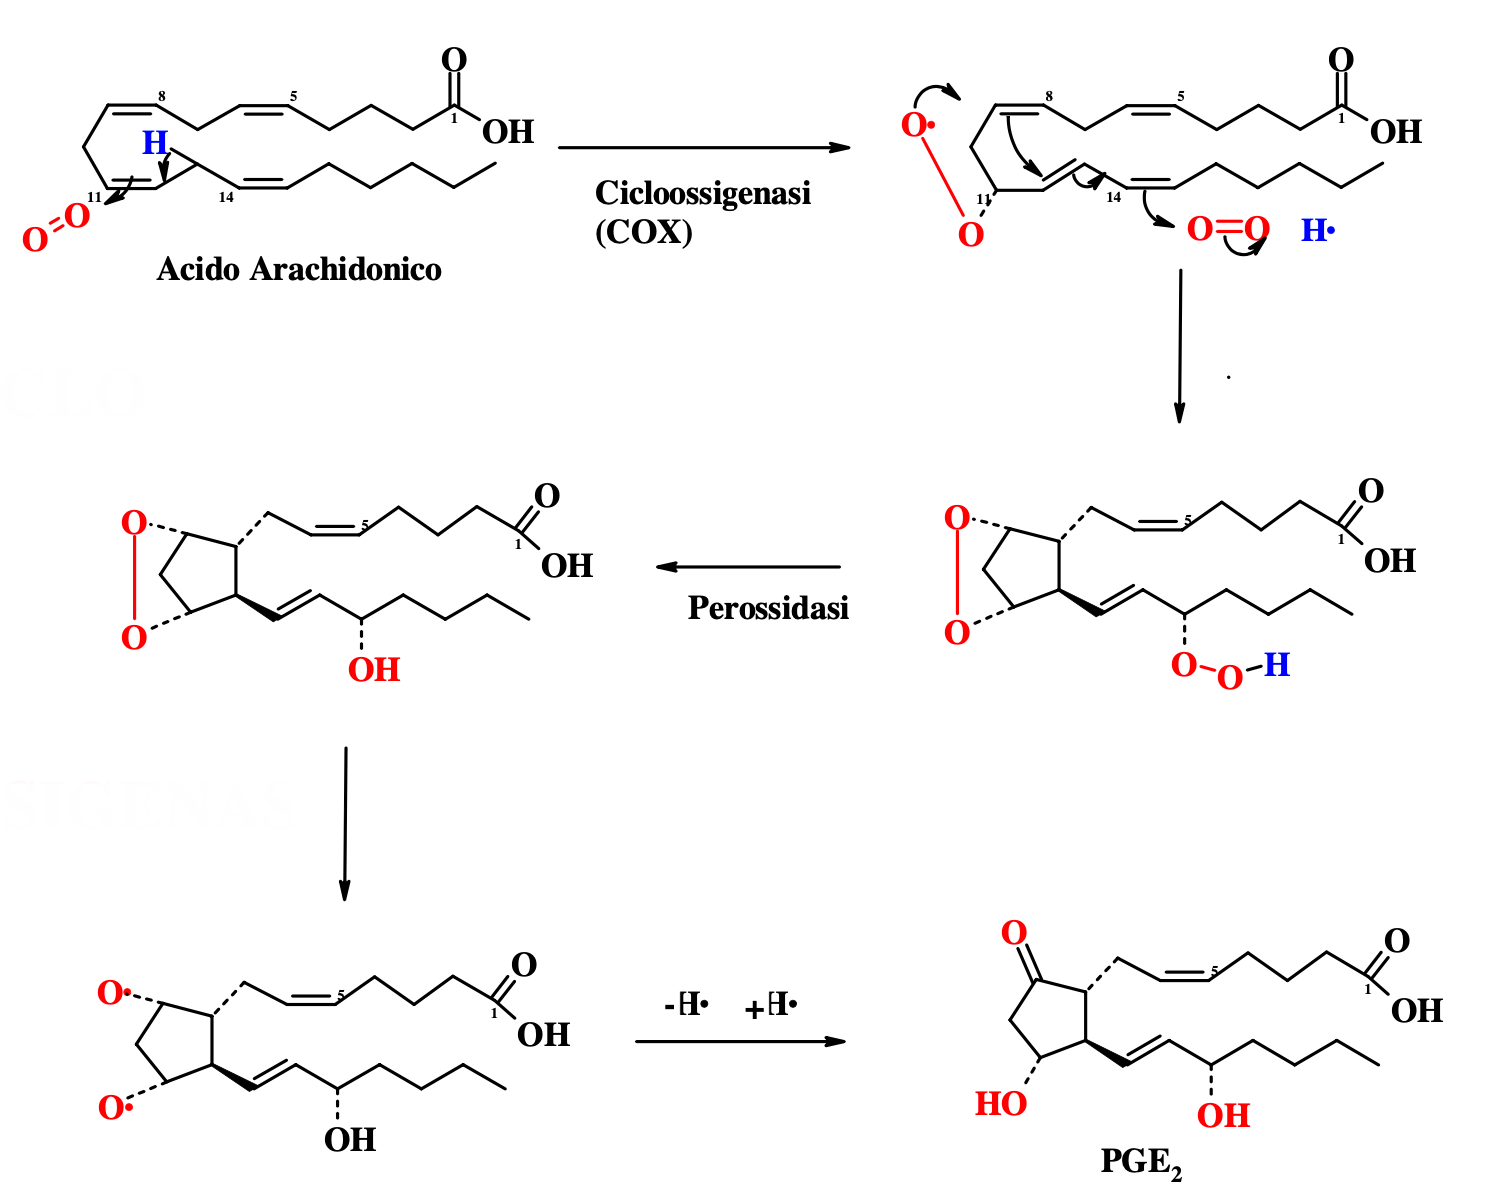
\includegraphics[width=\textwidth]{17_005}
\end{figure}

La reazione dell'acido arachidonico con il perossido forma un
endoperossido e di un idroperossido. La molecola viene chiamata
PGG\ped{2}. La PGG\ped{2} è un intermedio delle prostaglandine. La
ciclossigenasi ha anche un'azione di perossidazione, quindi dal
PGG\ped{2}, si forma PGH\ped{2}. In seguito si possono formare diverse
prostaglandine. Quella in reazione è la PGE\ped{2}.

Alcuni farmaci agiscono invece sulle lipossigenasi. Tuttavia, i FANS
vanno ad agire sulla ciclossigenasi per impedire la formazione di
prostaglandine, prostacicline e trombossani. Inibendo l'attività di
questo enzima, si inibisce la risposta infiammatoria, in quanto si va a
diminuire la sintesi dei mediatori responsabili dell'infiammazione.

\fullpicture*{17_004}{
I glucocorticoidi possono essere utilizzati per interrompere la liberazione dell'acido arachidonico dalla membrana cellulare. I glucocorticoidi sono dei derivati del cortisone, che è un ormone con delle funzioni biologiche. Questo comporta molti effetti collaterali e quindi vengono usati per stati patologici importanti
}

\section{FANS}

I FANS sono un ampio gruppo di farmaci, chimicamente differenti tra di
loro, che hanno come meccanismo d'azione comune, l'inibizione della
sintesi delle prostaglandine e di altri mediatori anti infiammatori.

In base al tipo di farmaco può essere più accentuata un'attività
rispetto ad un altra. Le attività principali sono:

\begin{itemize}
\item
\emph{Azione antinfiammatoria:} è dovuta all'inibizione dell'enzima
ciclossigenasi (COX), che regola la sintesi di prostaglandine,
prostacicline e trombossani. L'acido acetilsalicilico causa una
inibizione irreversibile, mentre gli altri FANS una reversibile.
\item
\emph{Azione antiaggregante:} è dovuta all'inibizione della sintesi di
trombossani a livello piastrinico. L'azione antiaggregante è
caratteristica dell'aspirina. Questo può essere un effetto
collaterale, specialmente in pazienti che hanno in corso altre
patologie.
\item
\emph{Azione analgesica:} si attua attraverso un meccanismo
soprattutto periferico, in quanto le prostaglandine aumentano la
sensibilità delle terminazioni nervose ai mediatori chimici del
dolore.
\item
\emph{Azione antipiretica:} si attua attraverso l'inibizione della
sintesi e liberazione della prostaglandina E\ped{2} da parte dei centri
termoregolatori dell'ipotalamo.
\end{itemize}

Il paracetamolo ha una spiccata attività antipiretica, rispetto a quella
antiinfiammatoria. Tuttora il motivo è sconosciuto.

\subsection{Ciclossigenasi}

La ciclossigenasi ha una struttura particolare in quanto è un omodimero.
Ciascuno dei monomeri presenta un sito catalitico che si trova
all'interno di una cavità particolare.

\marginpicture*{17_006}{Rappresentazione della ciclossigenasi. La membrana è rappresentata dalla parte azzurrina}

I due siti catalitici hanno entrambi le funzioni di formazione del
legame \ce{C-C}, sia l'attività perossidasica. Questo perché l'eme si
trova in prossimità del sito catalitico

\fullpicture{17_007}{Rappresentazione della ciclossigenasi con le varie strutture}{fig:HEME}

La macchina molecolare può essere vista nell'immagine \ref{fig:HEME}. Ciascun
dimero ha una porzione di proteina che si trova all'interno della
membrana cellulare. Ciascun monomero presenta un canale idrofobico,
attraverso il quale l'acido arachidonico entra nella macchina
molecolare. Appena entra, si trova in prossimità del sito catalitico.

La carbossigenasi ha due forme isomeriche, ovvero COX-1 e COX-2.
Inizialmente non si conosceva la COX-2, ma si pensava che fosse presente
solo una ciclossigenasi.

In certe specie, come nei cani, è stata osservata una terza forma di
ciclossigenasi, detta \emph{COX-3}. Si può quindi supporre l'esistenza
di una COX-3 umana, però non si hanno ancora delle conferme. Il
paracetamolo ha un'attività differente rispetto a quella degli altri
FANS, così come ha una struttura chimica differente, quindi potrebbe
avere un bersaglio differente.

Le due isoforme di COX sono molto simili tra di loro, infatti hanno un
peso molecolare simile (70 e 72 kDa) e sono omologhi, con il 65 \% nella
sequenza amminoacidica. Il sito attivo è molto simile.

Entrambe le COX sono omodimeri; il monomero presenta tre domini, che
sono stati identificati come:
\begin{itemize}
\item
\emph{EGF N-terminale}, che è un dominio
terminale presente in molte proteine. Funzionalmente non è molto importante
\item
\emph{Dominio di legame alla membrana}, che è formato da \alpha-elice, e permette ai due monomeri di essere a contatto con la membrana, creando il canale idrofobico per l'acido arachidonico
\item
\emph{Dominio del sito catalitico}, dove avvengono le reazioni. È caratterizzato per la vicinanza con l'eme.
\end{itemize}


Le immagini sono riferite alla COX-2.

La ricerca si è concentrata sugli inibitori delle COX-2, in quanto sono
presenti solo in presenza di uno stato infiammatorio. Questa
discriminazione è stata usata per limitare gli effetti collaterali.

La struttura della COX-2 è presente al URL
\url{https://www.rcsb.org/structure/5F19}.

In questa struttura è presente sia l'acido arachidonico, che dell'eme.
Andando a guardare la struttura in 3D, si vede la vicinanza dell'eme al
sito catalitico.

La COX-1 induce la formazione del muco che protegge lo stomaco e riduce
la secrezione gastrica. Quindi si ha un doppio effetto collaterale, in
quanto i FANS sono già acidi di per sé, inoltre viene inibita la
secrezione di muco. Quindi questo è un effetto collaterale importante,
però possono essere utilizzati con accortezza.

I FANS hanno delle strutture chimiche diverse tra di loro. In
particolare si hanno i salicilati, che sono dei derivati dell'acido
salicilico, il paracetamolo, che ha una struttura molto diversa rispetto
agli altri FANS.

Altri derivati sono quelli dell'acido propionico e dell'acido acetico.

Infine, si hanno gli inibitori selettivi della COX-2, che sono dei
diarileterocicli. Non sono molto utilizzati, in quanto il beneficio
della selettività verso COX-2 non è rilevante rispetto agli effetti
collaterali. Questo per dire che la ricerca di nuovi farmaci non dà
sempre i risultati sperati.


\subsection{Meccansimo d'azione dei FANS}

I FANS sono divisi in
classi\ft{Il meccanismo d'azione è simile per queste classi, però cambia un po'.}
in base a come riescono a inibire la COX. In particolare si hanno tre
classi:

\begin{itemize}
\item
\emph{Classe I.} Questo tipo di composti instaurano un inibizione di
tipo reversibile e competitiva con l'acido arachidonico stesso. Si ha
la formazione del complesso enzima-inibitore \[
\ce{E} + \ce{I} \ce{<=>} \ce{EI}
\] Un esempio di questa classe è l'ibuprofene
\item
\emph{Classe II.} Questa classe forma sempre un complesso
enzima-inibitore, che determina un cambiamento conformazionale. La
dissociazione del complesso è più lenta rispetto alla sua formazione
\[
\ce{E} + \ce{I} \ce{<=>} \ce{EI} \ce{<=>} \ce{EI*}
\] Le conseguenze di questo meccanismo sono che gli effetti
collaterali sono un po' più intensi, in quanto la dissociazione è
lenta e l'azione del farmaco dura di più Un esempio di questo farmaco
è l'indometacina.
\item
\emph{Classe III.} Questi composti formano un legame irreversibile con
la COX, quindi la disattivano completamente. Per far si che avvenga il
legame covalente, comunque è necessario avere un riconoscimento
non-covalente. Il legame covalente viene formato su un preciso
amminoacido. Questa classe ha un unico esponente, ovvero l'aspirina.
\[
\ce{E} + \ce{I} \ce{->} \ce{EI}
\]
\end{itemize}

\fullpicture*{17_008}{Alcuni FANS. Si nota che l'aspirina è stata scoperta a metà
dell'800. È un farmaco datato, ma che viene tuttora utilizzato.}

\section{Aspirina}

L'aspirina è stata scoperta nel 1897 da Felix Hoffmann. È stato il primo
FANS ad essere scoperto.

L'aspirina è un antiaggregante piastrinico, quindi rende il sangue più
fluido. Questo può essere un effetto collaterale, specialmente a lungo
termine, però può essere sfruttato per evitare la formazione di
trombi\ft{Questa preparazione prende il nome di ``cardioaspirina''} nel
sangue. Tra i due farmaci non cambia il principio attivo, ma la
formulazione, che permette di andare a interagire solo sulle COX
piastriniche.

A metà dell'800 si stavano cercando delle sostanze naturali che
potessero avere delle attività antinfiammatorie. Si scopre la salicina,
che viene isolata e purificata, estraendola dalla corteccia del salice.
È stata osservata una attività antinfiammatoria, ma con degli effetti
collaterali importanti.

Si scopre che, in vivo, la salicina viene trasformata ad acido
salicilico. Quindi è stato preso in considerazione quest'ultimo. Però
l'acido salicilico comunque manteneva le proprietà irritanti tipiche
della salicina.

A fine del 1800, Felix Hoffmann, un chimico della Bayer, ha cercato di
modificare l'acido salicilico, in modo tale da mantenere l'attività
antiinfiammatoria, ma rimuovendo le caratteristiche non volute
dell'acido salicilico. Quindi ha fatto un acetilazione dell'acido
salicilico, ottenendo così l'acido acetilsalicilico.

Il nome del farmaco \emph{aspirina} viene dal nome \emph{Spirea
ulmaria}, che è una pianta che è più ricca di salicina del \emph{Salix
alba}. La `a' iniziale viene da ``acetil'\,', che è la modifica
effettuata da Hoffmann.

Dopo aver scoperto il processo di produzione delle prostaglandine, si è
notato che l'aspirina va a bloccare questa sintesi. Il meccanismo di
reazione dell'aspirina sulla ciclocarbossigenasi è stato scoperto sono
nel 1970, dopo 70 anni dalla scoperta.

Negli anni '90 invece sono state scoperte le proprietà antitrombotiche
dell'aspirina.

Questo per dire che molti farmaci sono stati utilizzati senza conoscere
il meccanismo d'azione e nemmeno senza sapere su che pathway cellulare
agivano. Oggigiorno invece è necessario capire come un farmaco funziona,
per evitare effetti collaterali e quindi per investire meglio il
capitale della casa farmaceutica.

\marginpicture*{17_009}{Acido acetilsalicilico}

L'acido acetilsalicilico è molto solubile (\(\log P = 1.18\)) in quanto
presenta un gruppo carbossilico, che può deprotonarsi, e nemmeno nella
forma non carica, in quanto presenta due gruppi polari, ovvero un gruppo
estereo e un gruppo carbossilico. I due gruppi funzionali non sono
complanari e sono in posizione orto; anche questo è importante per la
funzione della molecola

\marginbox*{Il rapporto C/O è uguale a 2.5, che è basso, quindi la molecola, tendenzialmente, sarà solubile.}

La molecola contiene un ciclo aromatico, che sicuramente dona una certa
regolarità alla molecola. Questa parte della molecola è necessaria.

L'acido carbossilico conferisce una certa acidità alla molecola. Questo
acido carbossilico è necessario per la meccanica molecolare del farmaco.

Il peso molecolare è basso, quindi rientra nella categoria dei farmaci
che possono essere somministrati per via orale.

Il \(\log P\) consente alla molecola di distribuirsi sia in acqua, sia
nelle membrane, quindi si riesce a distribuire molto bene. L'acido
acetilsalicilico deve entrare nelle membrane e rimanerci, in modo tale
che le COX possano legarsi, quindi è necessaria anche un carattere
idrofobo.

\fullpicture*{17_010}{La COX può essere rappresentata in modo semplice. Un monomero
rappresenta la situazione senza l'acido acetilsalicilico, mentre
nell'altro è presente.}

In presenza dell'acido acetilsalicilico, una serina vicina al sito
catalitico viene acetilata, tramite reazione di transesterificazione.
Dopo aver legato il gruppo acetile nell'enzima, l'acido salicilico esce
dalla macchina molecolare. La reazione è rappresentata sotto; il gruppo
R indica la serina dell'enzima

\begin{figure}[H]
    \centering
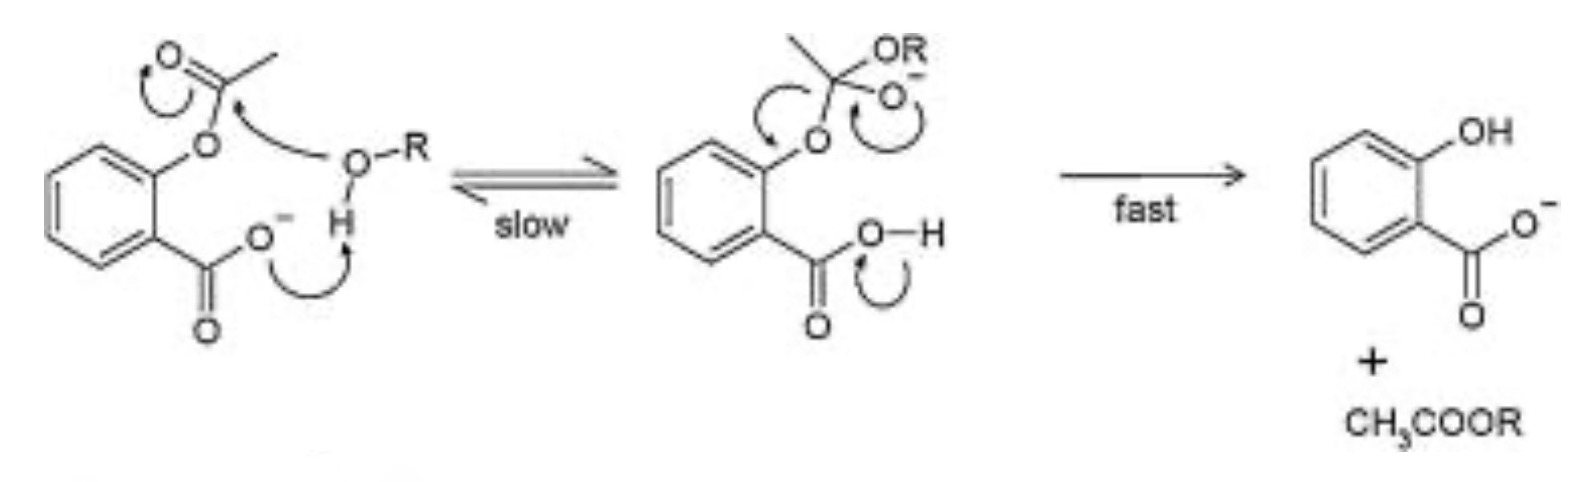
\includegraphics[width=\textwidth]{17_011}
\end{figure}

Avvenne l'attacco nucleofilo al carbonio del carbonile. L'acido
carbossilico deve essere in forma ionica, per poter legare l'\ce{OH}.
Questo meccanismo si chiama \emph{assistenza del gruppo funzionale
vicinale}. Questo serve per favorire la deprotonazione dell'ossidrile,
il che lo rende un buon nucleofilo.

Si forma l'intermedio tetraedrico e poi avviene una rapida eliminazione
del gruppo uscente. Il gruppo uscente è un gruppo fenilico, che è un
buon gruppo uscente e questo rende la reazione molto veloce.

Si forma quindi l'acido salicilico, mentre il gruppo acetile rimane
attaccato alla serina della COX.

La vicinanza dei gruppi è necessaria affinché la reazione avvenga. Se il
gruppo \ce{OH} fosse in meta o in para, il gruppo funzionale non sarebbe
utile in quanto non riuscirebbe deprotonare il gruppo ossidrilico della
serina.

L'acetilazione della serina impedisce all'acido arachidonico di entrare
nel sito catalitico, quindi non può essere processato

\fullpicture*{17_012}{La COX, in questa immagine, contiene l'acido acetilsalicilico,
che si localizza nella stessa zona.}

L'acido arachidonico deve disporsi in un modo preciso per essere
processato. L'acido acetilsalicilico crea un blocco che non permette
all'acido arachidonico di entrare e di arrivare al sito catalitico.

\fullpicture*{17_013}{Ingrandimento della regione del sito catalitico. Questo è il
prodotto finale di transesterificazione che viene a crearsi in seguito
all'acetilazione della Ser-530.}

Un altro aspetto importante dell'acido acetilsalicilico è la durata
d'azione, in quanto la modifica operata è covalente. Le cellule devono
risintetizzare la macchina molecolare, quindi la durata dell'effetto
farmacologico dipenderà dal tempo che necessita la cellula.

Le cellule con il nucleo impiegano poche ore per risintetizzare questa
macchina molecolare, quindi gli effetti durano poche ore. Le piastrine,
che sono cellule senza nucleo, però impiegano più tempo per ricostruire
la macchina molecolare, quindi l'effetto antiaggregante persista per
alcuni giorni.

L'acido acetilsalicilico è un inibitore non selettivo quindi agisce sia
sulle COX-1, che sulle COX-2. Questo determina gli altri effetti
collaterali, come le ulcere.

\section{Derivati dell'acido propionico}

L'aspirina causa una modifica irreversibile, quindi causa degli effetti
collaterali importanti. Le case farmaceutiche sono andate a cercare
delle molecole che potessero andare a sostituire l'aspirina, sia da un
punto di vista meccanicistico, sia dal punto di vista degli effetti
collaterali.

\marginpicture*{17_014}{Acido propionico}

Questa categoria di farmaci ha una buona efficacia e gli effetti
collaterali sono leggermente diversi. Gli effetti sono comunque
tollerabili.

\subsection{Ibuprofene}

L'ibuprofene è un farmaco derivato dall'acido propionico, infatti il
suo nome è \emph{i}so\emph{bu}til-\emph{pro}pionic acid \emph{fen}ile.

\marginpicture*{17_015}{Ibuprofene}

Questo farmaco ha ancora una buona attività e delle buone
caratteristiche tali da sostituire l'aspirina. È un inibitore non
covalente, infatti si rimuove la componente esterea dell'acido
acetilsalicilico.

L'acidità è simile a quella dell'aspirina \(pK_a = 5.30\), però è
necessario togliere l'estere in quanto si vuole avere una modifica
reversibile.

È un farmaco discretamente recente, in quanto è stato brevettato nel
1961.

La molecola presenta un gruppo isobutilico, che può dare interazioni
idrofobiche. Si mantiene il gruppo carbossilico. È stato mantenuto il
ciclo aromatico, dove i leganti sono in posizione 1 e 4.

Il rapporto C/O è pari a 6.5, è molto elevato. Quindi questa molecola
può avere dei problemi dal punto di vista della solubilità. Quindi la
molecola ha delle interazioni idrofobiche intense, però questa
caratteristica può essere utile, in quanto i farmaci, una volta
raggiunta la membrana, rimangono lì. Questo consente di aumentare la
disponibilità del farmaco. Il peso molecolare è 206, mentre il
\(\log{} P\) è pari a 3.97, che indica che la molecola resta nella
membrana.

Il problema della solubilità di questa molecola viene superata grazie
alle formulazioni; questo avviene perché la molecola è molto
interessante dal punto di vista farmaceutico.

Ogni volta che si ha un centro chirale, un chimico farmaceutico deve
separare i due enantiomeri e deve cercare di capire se una delle due
specie ha un'attività maggiore, se è tossica, oppure se la miscela
racemica è altrettanto efficace.

Nel caso dell'ibuprofene, si è visto che la forma attiva è quella S,
però la formulazione prevede una miscela racemica. In questo caso, si
tiene la miscela racemica, in quanto perché la forma R, quando viene
assorbita, viene isomerizzata dall'\emph{racemasi acetil-CoA-dipendente}
all'isomero S. Questo evento non è comune per gli altri farmaci, ma è
peculiare dell'ibuprofene.

\marginbox*{
    Solo la forma S è attiva, mentre la R viene convertita nella forma S.
    R non è attivo, però non si può considerare inattivo in quanto viene riconvertito in S.
}

La struttura della COX a cui l'ibuprofene è legato è rappresentata nell’immagine
 \ref{fig:IBU}. Si vede che l'ibuprofene è localizzati vicino al sito
catalitico e compete reversibilmente con l'acido arachidonico.

Le interazioni che avvengono nella tasca sono solitamente idrofobiche,
però possono esserci anche delle interazioni idrofiliche, che permettono
di avere delle interazioni specifiche con i farmaci.

Nel caso dell'ibuprofene, la porzione isobutilica si trova in una
regione idrofobica, che favorisce la molecola a restare nella cavità,
mentre l'altra porzione viene posizionata in prossimità di una Tyr e di
una Arg.

\fullpicture{17_016}{Ibuprofene nel sito catalitico della COX}{fig:IBU}

La stabilizzazione all'interno della cavità idrofobica è sostenuta da
legami importanti, che permettono un buon riconoscimento in questa
zona.

\section{Derivati dell'acido acetico}

\subsection{Indometacina}

L'indometacina presenta un anello \emph{indo}lico, come struttura di
regolarità (rispetto al benzene). Inoltre, presenta un gruppo
\emph{met}ossile, che permette le interazioni idrofobiche però permette
una certa solubilità in acqua.

\marginpicture*{17_017}{Indometacina}

La funzione acida viene mantenuta ed è vicina al centro di regolarità,
però cambia la distanza in quanto si aggiunge un linker. Infine, è
presente una ammide, formata da un derivato dell'acido benzoico (acido
4-cloro-benzoico) e dall'azoto indolico. Questa struttura dà delle
interazioni idrofobiche e quindi va a sostituire la funzione del gruppo
isobutilico nell'ibuprofene.

Il \(\log{} P\) è uguale a 4.27 e quindi si è al limite della
solubilità, che è pari a 5. C'è comunque un miglioramento rispetto
all'ibuprofene, che è più alto. Questo, come nel caso dell'ibuprofene, è
una caratteristica favorevole, in quanto la molecola si dispone più
facilmente nelle membrane. Questo consente più interazioni con l'acqua,
nonostante la molecola abbia un certo carattere idrofobico. Le funzioni
che possono interagire con l'acqua sono disposte in tutta la molecola,
specialmente intorno al nucleo aromatico.

Nell'ibuprogene invece, solamente una piccola regione può reagire con
l'acqua, mentre il resto della molecola ha un carattere idrofobo.

\fullpicture{17_018}{Interazioni dell'indometacina nel sito catalitico delle COX}{fig:IND}

Come si vede nell'immagine \ref{fig:IND}, l'indometacina si dispone vicino al sito catalitico delle COX, e quindi
blocca l'ingresso dell'acido arachidonico, per competizione. In questo
caso, la competizione avviene con una dissociazione del complesso
enzima-inibitore più lenta. Questo determina delle caratteristiche di
azione del farmaco diverse.

Gli effetti collaterali saranno più importanti, come l'azione del
farmaco. Questo può essere superato tramite l'utilizzo di formulazioni
localizzate, come creme, che consentono una somministrazione
localizzata, in quanto questo farmaco è potente, e si vogliono attenuare
gli effetti collaterali.

Anche in questo caso, le interazioni dell'indometacina nella cavità
idrofobica sono specifiche. Si ha ancora la stessa interazione con l'Arg
e con la Tyr. Le interazioni idrofobiche del metossile sono rivolte
verso una Val. Il nucleo aromatico planare, l'indolo, ha una interazione
idrofobica con una seconda Val.

\fullpicture*{17_019}{
Interazioni dell'indometacina e dell'ibuprofene rispetto ai due
gruppo carbossilati; questi gruppi sono sovrapposti, quindi si hanno le
stesse interazioni con la macchina molecolare.
Il clorobenzile dell'indometacina è sovrapposto all'isobutile
dell'ibuprofene. Quindi le due molecole sono complementari alla macchina
molecolare.\\L'ampiezza dell'anello indolico è maggiore rispetto a quello benzenico,
quindi nell'indometacina il canale è stato allargato. Esiste una tasca,
molto particolare, che permette di distinguere la COX-1 e la COX-2.\\L'unica differenza strutturale tra le due sta proprio nella forma della
cavità idrofobica, che permette di avere delle interazioni specifiche.
}

\paragraph{Ketorolac}

Questo è un farmaco molto potente, che può avere degli effetti
collaterali importanti. Ha degli effetti analgesici comparabili a dei
derivati della morfina, che agiscono a livello cerebrale, anche se il
meccanismo d'azione riguarda sempre l'inibizione della COX.

\marginpicture*{17_020}{Ketorolac}

\clearpage

\section{Altri farmaci}

Altre molecole che fanno parte dei FANS, ma non hanno strutture simili a
quelle viste prima sono la Nimesulide. Questa molecola ha degli effetti
collaterali a livello gastrico minori, però, a lungo termine, dava dei
danni a livello epatico importanti.

\marginpicture*{17_021}{Nimesulide}

È ancora disponibile, però è necessaria la ricetta medica per poterlo
usare.

\subsection{Paracetamolo}

Il paracetamolo fa parte dei derivati para-amminofenolici, ed è l'unico
di questa classe di farmaci che viene ancora usato. Gli altri farmaci
hanno dimostrato una tossicità a livello epatico molto elevata.

\marginpicture*{17_022}{Paracetamolo}

È uno dei farmaci che si utilizzano con più facilità, in quanto ha una
tollerabilità molto elevata, mentre gli effetti collaterali sono
ridotti. La tossicità è bassa.

Ci sono delle formulazioni diverse. Ad esempio esistono le compresse con
1000 mg di paracetamolo, che è molto. Questo farmaco, in dosi elevate,
porta ad una tossicità epatica.

Questa molecola ha una spiccata attività analgesica e antipiretica,
mentre l'attività antinfiammatoria è bassa.

Per questo farmaco non è ancora chiaro il meccanismo d'azione; si è
visto che inibisce prevalentemente le COX presenti a livello del SNC. Le
proposte di un possibile meccanismo d'azione sono:

\begin{itemize}
\item
È presente una terza forma di COX (nell'uomo), con cui il paracetamolo
interagisce
\item
L'inattivazione della macchina molecolare avviene tramite ossidazione
del paracetamolo, quindi la macchina molecolare si riduce.
\end{itemize}

Nonostante il meccanismo di reazione non sia noto, è ampiamente usato
per trattamento di stati febbrili e per le malattie esantematiche. Questo
per dire che è un farmaco sicuro.

Questo farmaco, vista la tossicità epatica elevata, possiede un
antidoto.

\marginbox*{
Queste informazioni sono ottenute tramite le prime sperimentazioni di
questi farmaci. Se una persona è già compromessa al fegato, è necessario
tenerla sotto controllo.
}

Il paracetamolo, quando viene metabolizzato a livello epatico, viene
metabolizzato in un intermedio chinonico, che è tossico e deve essere
metabolizzato molto velocemente.

Questa metabolizzazione avviene tramite
una reazione con il glutatione a livello epatico. La disponibilità di
glutatione non è elevata, quindi se si assume una quantità elevata di
paracetamolo in tempi rapidi, questa via metabolica non funziona più.

L'intermedio tossico può reagire con le proteine epatiche, che
contengono dei gruppi tiolici, legandosi ad esse.

Come antidoto si usa l'N-Acetilcisteina, che è un donatore di radicali
sulfidrilici, che vanno a neutralizzare il metabolita tossico.

\begin{figure}[H]
    \centering
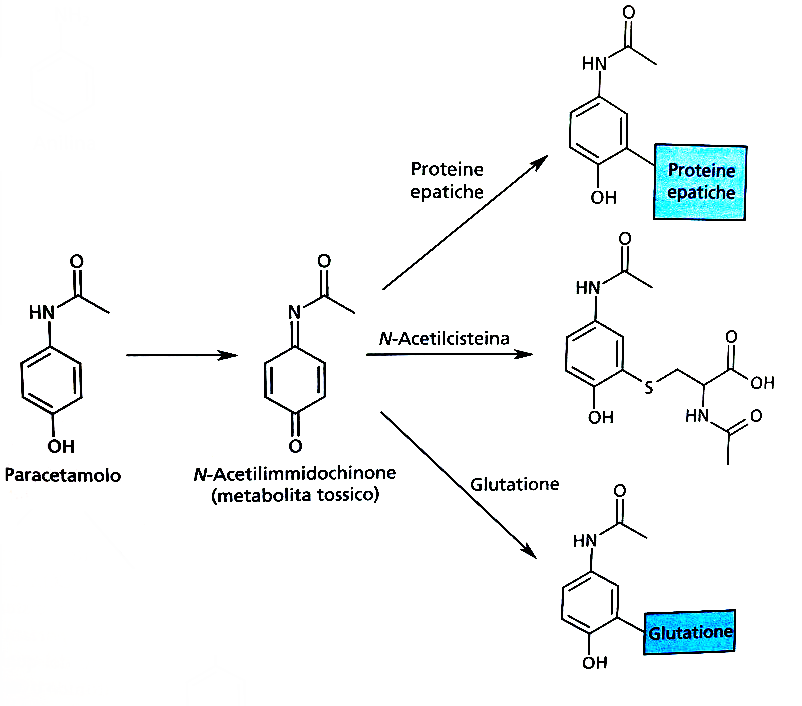
\includegraphics[width=0.8\textwidth]{17_023}
\end{figure}

\clearpage

\subsection{Inibitori delle COX-2}

Visti gli effetti collaterali dei FANS, si è ricercato un inibitore
selettivo della COX-2, che è presente solo se c'è uno stato di
infiammazione

\fullpicture*{17_024}{Alcuni farmaci sono più selettivi per la COX-1, altri per la COX-2. In realtà, i farmaci sono tutti inibitori non selettivi.}

Sono state sviluppate delle molecole che riescono a inibire sono le COX
presenti nei macrofagi. I macrofagi sono responsabili dei mediatori
dell'infiammazione. Le COX dei macrofagi sono COX-2, però al tempo, non
si sapeva della distinzione tra i due enzimi.

Gli inibitori delle COX-2 non hanno gli effetti collaterali legati
all'inibizione delle COX-1. Non avendo l'inibizione dell'aggregazione
piastrinica, gli inibitori delle COX-2 hanno altri effetti collaterali,
molto peggiori degli effetti collaterali a livello gastrico, ovvero
portano alla formazione di trombi e presentano anche una certa
cardiotossicità. Questo perché non c'è più l'equilibrio di inibizione
tra COX-1 e COX-2.

Quando è stato scoperto il meccanismo d'azione dei FANS, si è anche
scoperta la presenza di due COX. La purificazione degli enzimi è stato
un processo lungo, però nel 1991 è stata confermata l'esistenza dei due
isomeri dell'enzima.

\marginpicture*{17_025}{DuP-697}

La ricerca è partita dal composto in figura. Questo composto è un diaril
eterociclico, con una catena laterale in para. Questo composto è stato
il punto di partenza per la sintesi dei farmaci selettivi, una volta
scoperte le strutture delle COX.

In soli 8 anni sono stati messi in commercio due farmaci, ovvero il
Celecoxib e il Rofecoxib. Si è visto che gli effetti collaterali erano
molto intensi, e questo ha portato al ritiro dal commercio di un
farmaco, il Vioxx. Il Celecoxib è ancora in commercio, però viene usato
solo sotto supervisione medica.

Qeesti farmaci sono stati sviluppati per pazienti con dei problemi a
livello gastrico, che quindi non possono assumere i FANS. Questi farmaci
non sono di uso comune, però sono disponibili quando il compromesso
attività-effetto collaterale è positivo per il paziente.

\subsection{Celecoxib}

Il Celecoxib ha una struttura simile alla molecola di partenza; però
questo un farmaco.

\marginpicture*{17_026}{Celecoxib}

La struttura del farmaco non presenta il gruppo COOH. La struttura
ricorda l'indometacina, perché la struttura regolare è formata da un
ciclo a cui è legato un altro ciclo.

Questo farmaco può essere utilizzato per via orale perché il
\(\log{} P\) rientra tra i parametri, infatti è pari a 3.53.

\fullpicture*{17_027}{Sovrapposizione del sito catalitico COX-1 e COX-2. Le
differenze sono minime}

La tasca polare del sito catalitico presenta una variazione; nella COX-1
c'è una His-513, mentre nella COX-2 è presente una Arg-513.

L'arginina permette di avere una tasca un po' più grande della COX-2,
rispetto alla COX-1. Quello che rende più accessibile la tasca è la
differenza nella posizione 523, dove la COX-1 ha legato una isoleucina,
mentre la COX-2 ha legato una valina.

Queste differenze sono minime variazioni tra i siti catalitici, che
determinano la possibilità degli inibitori selettivi COX-2 quando si è
in presenza della tasca idrofobica più ampia e più accessibile

\fullpicture*{17_028}{La COX-1 presenta una isoleucina che chiude la tasca
idrofobica, mentre nella COX-2 si ha una valina che permette di avere
una cavità più ampia e più accessibile.\\Nel momento in cui si ha la somministrazione degli inibitori
non selettivi, in entrambi i casi si fermano prima di trovare la tasca.
Quindi si ha l'interazione del gruppo carbossilico a livello di
arginina-120, in entrambi i casi. Quindi i composti non sono selettivi.}

Negli inibitori delle COX-2, la molecola riesce ad andare oltre e riesce
a mettere la catena in para all'interno della tasca idrofobica, in cui
si ha un gruppo funzionale che interagisce in modo consistente (tramite
legame a idrogeno) con la Arg-513, che invece è tipica della COX-2.

Il sostituente in para va a dare anche interazioni specifiche, sempre
con legami ad idrogeno con Arg, Ser e Leu, che compongono la cavità
della COX-2.

\fullpicture*{17_029}{Rappresentazione della COX-2 con legato il Celecoxib.}

\fullpicture*{17_030}{Rappresentazione dell'interazione tra il sostituente in para e la tasca idrofobica.}

\fullpicture*{17_031}{Sovrapposizione dell'ibuprofene e del Celecoxib nel sito delle
COX-2. L'inibitore selettivo delle COX-2 ha la capacità di occupare la
tasca in modo selettivo.}
